
\chapter{Experimental Setup}

This chapter describes the experimental setup used in this study.  For the sake of brevity, brief descriptions of the Large Hadron Collider (LHC), the Compact Muon Solenoid (CMS) and its  subdetectors are provided. Also, it is shown how  the high-level physics objects are processed and reconstructed.

\section{The Large Hadron Collider}

The Large Hadron Collider (LHC) is the world largest and powerful particle accelerator for protons and heavy-ions ever build. It is located in a complex of other accelerator operated by the European Organization for Nuclear Research (CERN), in the border of between Switzerland and France. The LHC is built in the same 26.7 km extension tunnel with depth varying from 45 m to 170 m below the surface (the LHC plane is tilted 1.4\% for construction reasons), once used by Large Electron–Positron Collider. The CERN complex is a composition of many accelerators, for proton and heavy-ions, used to provide beams of particles for smaller experiments and as a sequence of injectors for the LHC. Figure~\ref{lhc_complex} presents the many components of the LHC complex of accelerators. A detailed description of the LHC can be found at~\cite{Evans:2008zzb, Bruning:782076, Bruning:815187, Benedikt:823808}.

% lhc complex
\begin{figure}[htbp]
    \centering
    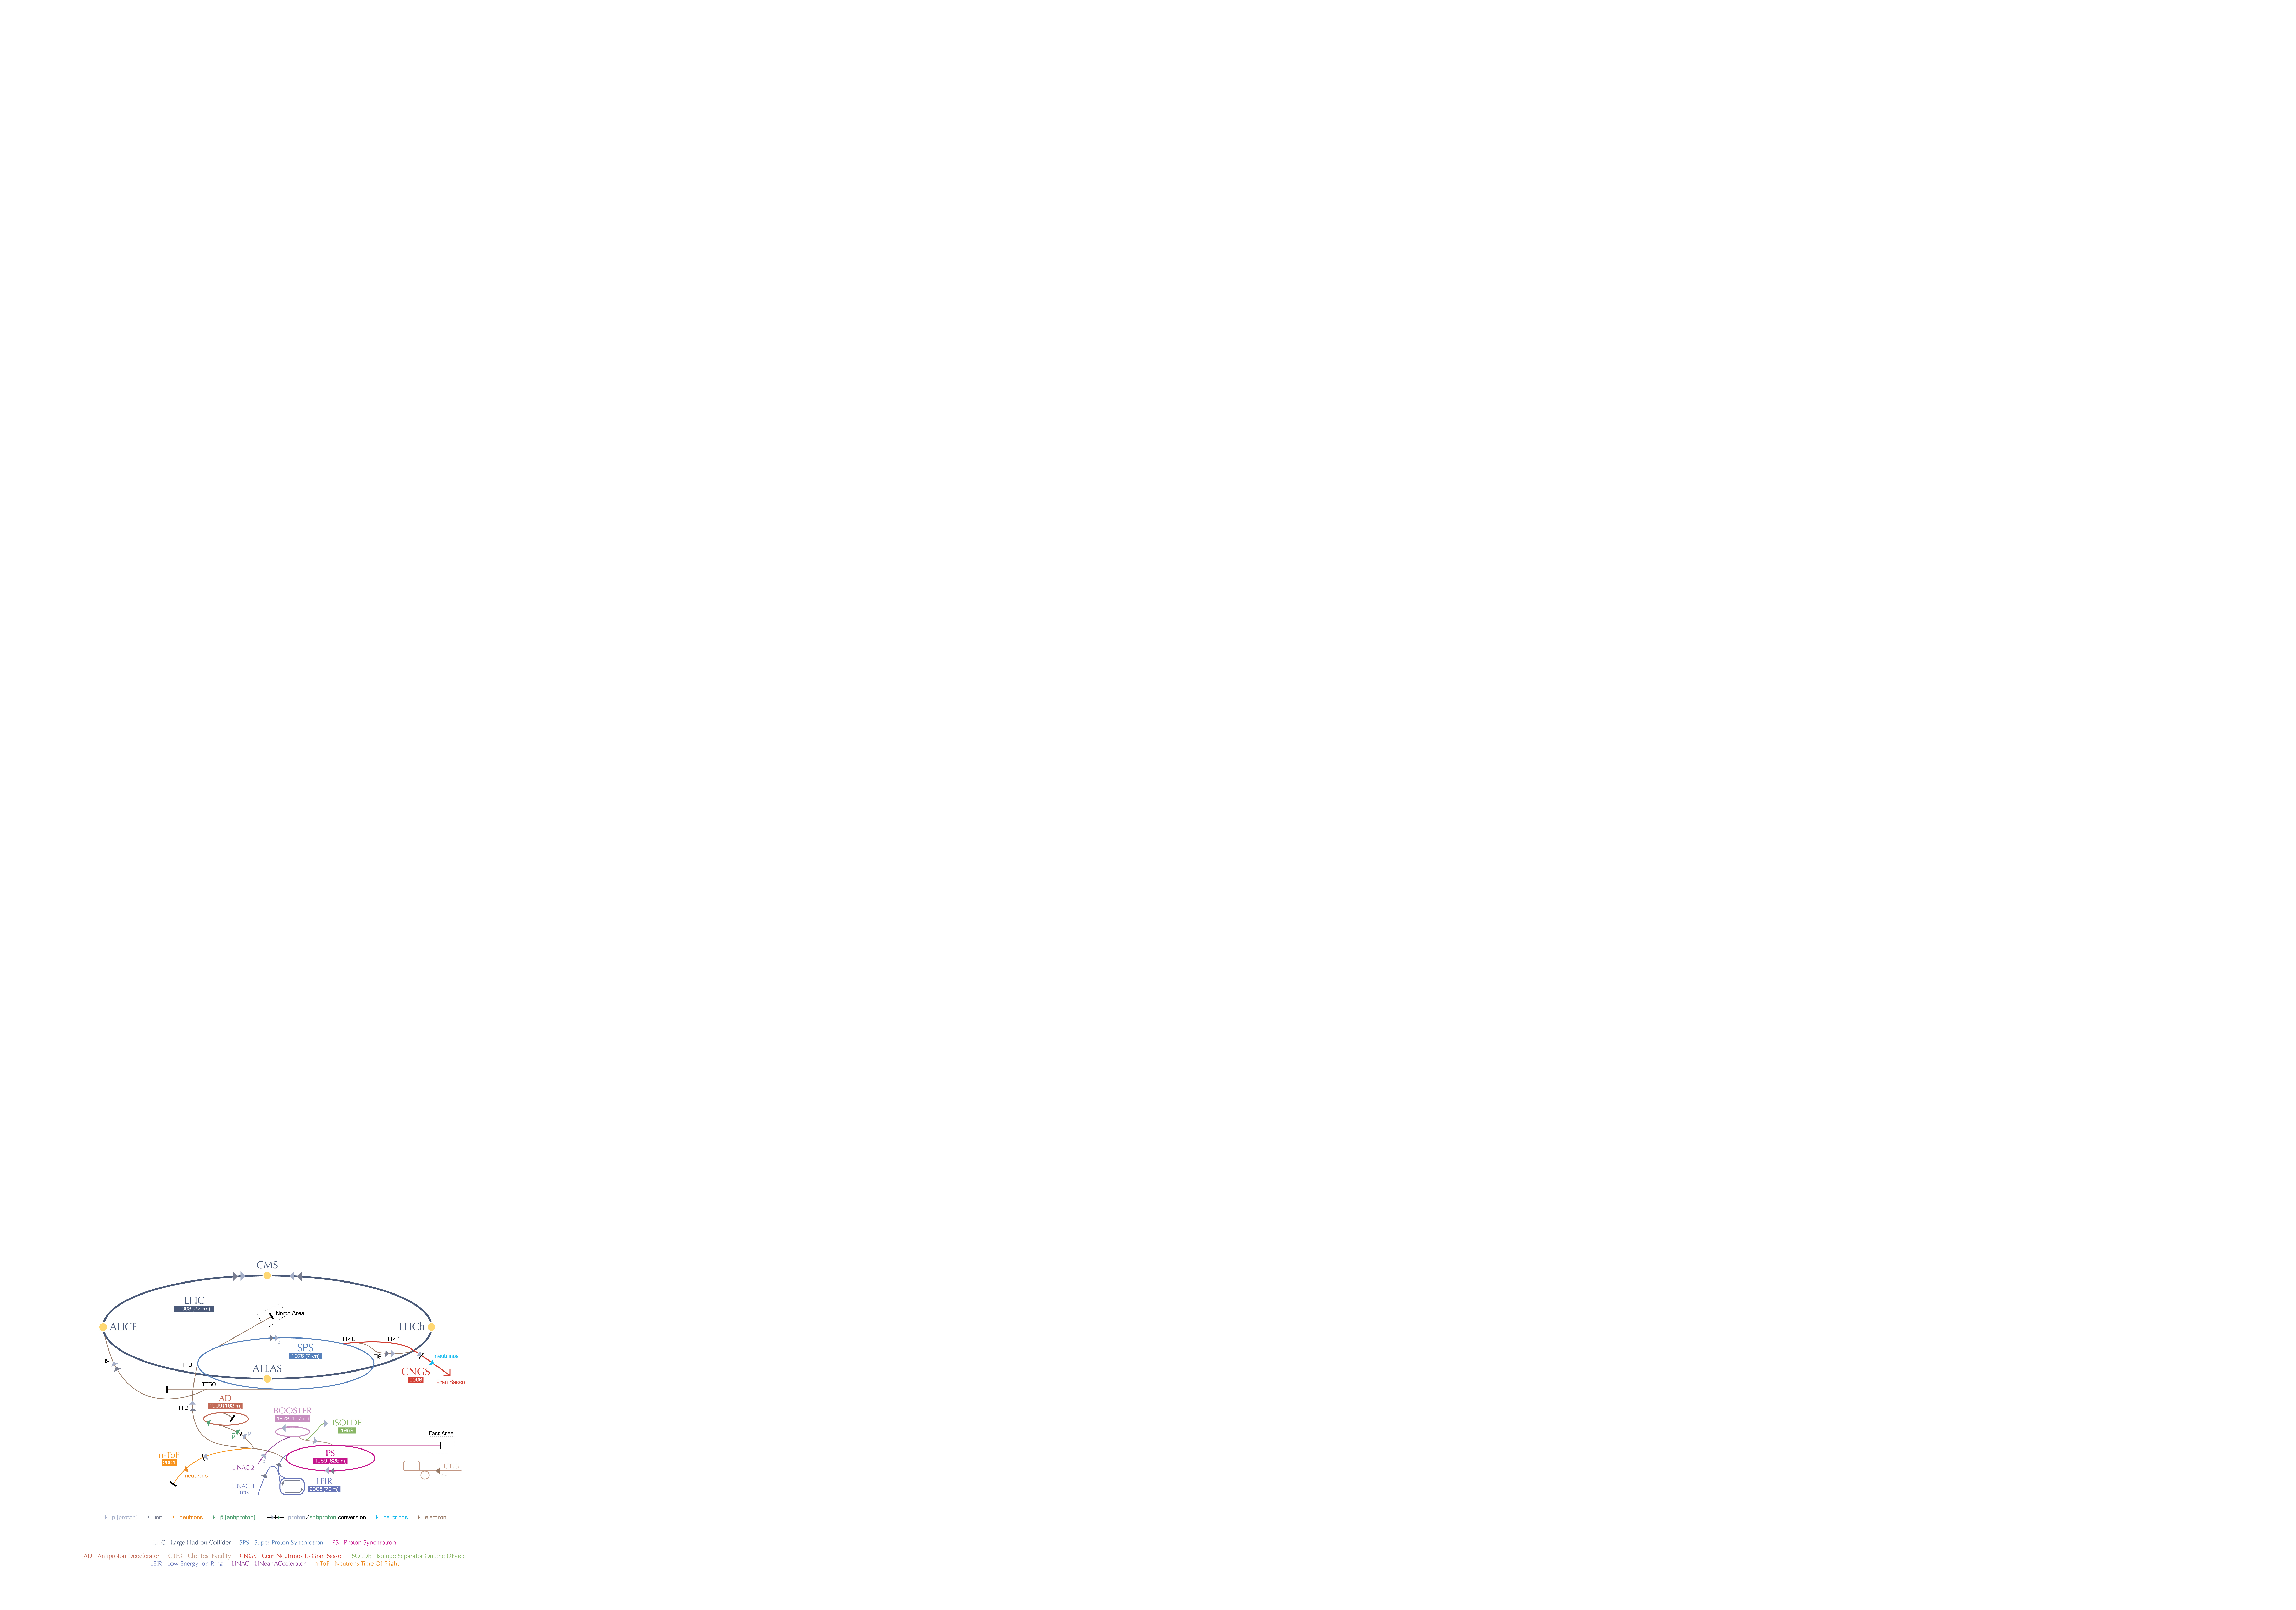
\includegraphics[width=\textwidth]{figures_and_tables/experimental_setup/lhc_complex.pdf}
    \caption{The LHC is the last ring (dark grey line) in a complex chain of particle accelerators. The smaller machines are used in a chain to help boost the particles to their final energies and provide beams to a whole set of smaller experiments. Source:~\cite{lhc_complex}.}
    \label{lhc_complex}
\end{figure}

A LHC section is composed of two vacuum pipes, in which the bunch of particles travels in opposite directions. This means that both beams are magnetically coupled by the same super-conducting magnetic system, saving space and allowing the use of the pre-built LEP tunnel. The particle acceleration is made by Resonant Cavities~\cite{Baird:1017689}. Those cavities apply to each beam a set of radio-frequencies (RF) used to transfer energy by means of a 2 MV electric potential per cavity, at a revolution frequency of 400.789 MHz. The acceleration is applied to bunches of particles. The bunch configuration depends of the injection mode (configurable), but a typical $pp$ injection would be composed by 2808 bunches of $1.1 \times 10^{11}$ protons each. Proper timing of the bunches injection and the RF is a key factor for an efficient energy transfer inside the RF cavities. The cavities also are operated in low temperatures of 4.5 K, to ensure superconducting properties and reduce energy losses.

The nominal time spacing between each bunch (bunch crossing - BX) is 25 ns. This defines the clock frequency of the LHC at $f_{LHC} = 40$ MHz. This frequency is propagated to all experiments and used as a reference for timing and synchronization. 

In certain positions, called the interaction points (IP), those two bunches are allowed to cross, possibiliting the particle collisions. The experiments on the LHC are located in those interaction points. ATLAS (A Toroidal LHC ApparatuS)~\cite{atlas_collaboration_2008} and CMS (Compact Muon Solenoid, better explained in the next section), at P1 and P5, respectively, are so called general proposes experiments, with focus on different aspects of a particle interactions in the LHC energy scale, including extensive test of known Standard Model process (in high and low transverse momentum regime), including the Higgs sector and Heavy Flavour Physics (phenomena involving the hadrons composed by $c$ and $b$ quarks), exploration of Beyond Standard Model (BSM) phenomena, as well as an competitive program in heavy-ions collisions. The LHCb (Large Hadron Collider beauty)~\cite{Alves:2008zz} is a experiment devoted, mostly, to precision measurements of CP violation and rare decays of $B$ hadrons. The ALICE (A Large Ion Collider Experiment)~\cite{Aamodt:2008zz} experiment is dedicated to the study of $p$-$Pb$ and $Pb$-$Pb$ collisions and processes such as QCD, strongly interacting matter and the quark-gluon plasma at extreme values of energy density and temperature.

The number of events of a certain kind $i$, per unit of time, is given by Equation~\ref{events_rates_cross_section}.

\begin{equation}
    \frac{dN^{i}}{dt} = \sigma^{i} \mathcal{L},
    \label{events_rates_cross_section}
\end{equation}
where $\sigma^{i}$ is the cross-section for a certain process $i$ and $\mathcal{L}$ is the instantaneous luminosity delivered by the LHC.

 In order to accumulate as much statistics as possible, in the shortest amount of time (for the most efficiently use of the resources available, including person-power), the luminosity is a key factor in the exploration of the collisions. This is dependent of the number of particles per bunch, number of bunches per beam, revolution frequency, form factors of the bunches, crossing angles at the interaction points and correction factors to address relativistic and electromagnetic associated phenomena. For $pp$ collisions, the LHC aims peak luminosities of, for ATLAS and CMS, around $2x10^{34} cm^{-2}s^{-1}$. For future upgrades of the LHC (called HL-LHC~\cite{ApollinariG.:2017ojx}), the peak luminosity might increase 10 times, allowing an accumulated luminosity~\footnote{Accumulated (or integrated) luminosity is defined as $L = \int \mathcal{L}\text{ }dt$.} of 3000 $fb^{-1}$.

 The LHC can collide protons with center-of-mass energy $\sqrt{s}$ up to 14 TeV. Different energy configurations have been used so far, historically increasing the energy. For the operation cycle used in this study (Run2, from 2015 to 2018), the machine was producing collisions at $\sqrt{s} = 13$ TeV. For the next operation cycle (Run3), to start in 2022, it is expected that the LHC might reach the 14 TeV energy values.